\documentclass[14pt,final]{report}
% \usepackage[english,russian]{babel}
\usepackage{wrapfig}
\usepackage{caption}
% TODO: Do something 
% https://www.overleaf.com/read/fkzbbcxxrxvz
% This was edited locally
% And this was edited on the server

% \RequirePackage{polyglossia}
% \setotherlanguage{english}
% \setdefaultlanguage{russian}

\RequirePackage[times,firacode,a4paper,microtyping,732,smalltitles,listbib,lmmath]{subook}
% \RequirePackage[times,firacode,a4paper,microtyping,handbook,smalltitles,listbib]{subook}
\RequirePackage{tabularx}
% \RequirePackage{grphicx}
\graphicspath{{pics/}}

% \usepackage{showframe}
\addto\captionsrussian{\renewcommand{\figurename}{\textbf{Рисунок}}}
\captionsetup[figure]{labelsep=period}
\captionsetup[figure]{labelfont=bf}

% pygmetize
\RequirePackage{minted}
\usemintedstyle{tango} % bw

% \setmainfont{Times New Roman}
\setcounter{subsection}{1}
\begin{document}
\thispagestyle{empty}
\begin{center}
МИНИСТЕРСТВО ОБРАЗОВАНИЯ И НАУКИ РОССИЙСКОЙ ФЕДЕРАЦИИ

Федеральное государственное бюджетное образовательное учреждение высшего образования

«ИРКУТСКИЙ  ГОСУДАРСТВЕННЫЙ УНИВЕРСИТЕТ»\\
(ФГБОУ ВО «ИГУ»)
\end{center}
\vfill % \vfil \vfill \vfilll

\noindent\begin{tabularx}{\textwidth} {
  >{\raggedright\arraybackslash}X
  >{\raggedright\arraybackslash}X }
Институт математики и информационных технологий
&
Кафедра информационных технологий
\end{tabularx}

\vfill
\begin{center}
  \textbf{ОТЧЕТ}
\vspace{1em}

о курсовой работе по курсу <<Разработка WEB-приложений>>

{\bf Разработка дизайна мессенджера}

\end{center}
\vfill

\noindent\begin{tabularx}{\textwidth} {
  >{\raggedright\arraybackslash}X
  >{\raggedright}X }
&

Студента 3 курса группы 2371\\
Казаева Вадима Андреевича\\
Направление\;: 02.03.02~--~Фундаментальная информатика и информационные технологии\\[2em]

Руководитель:\\
доцент\\
Черкашин Евгений Александрович\\[2em]

Курсовая работа защищена с оценкой\\[1em] \underline{\hspace{3cm}}
\end{tabularx}
\vfill
\begin{center}
  Иркутск -- 2021
\end{center}
\clearpage

\tableofcontents

\chapter*{ВВЕДЕНИЕ}
% TODO: Add contents line
\label{chap:intro}
\section*{Актуальность темы}
Сейчас, как никогда, компании должны взаимодействовать со своей аудиторией через каналы, которые предпочитают клиенты. Наблюдается большой рост популярности систем самообслуживания и в частности – использования мессенджеров для решения возникающих вопросов. Обмен сообщениями является самой быстрорастущей и наиболее широко используемой формой межличностного общения. Асинхронное взаимодействие позволяет клиенту выбрать то время, которое удобно ему.\\
\section*{Цели и задачи работы}
\textbf{Целью} данной работы является разработка дизайна WEB-мессенджера.
\\
Для достижения поставленной цели необходимо решить следующие \textbf{задачи}: \\
1) Проанализировать требования к web-мессенджеру; \\
2) Разработать структуру и дизайн web-мессенджера; \\
3) Выполнить реализацию разработанных макетов. \\
\newline
Согласно требованиям предмета, WEB-мессенджер должен быть выполнен на основе
JavaScript-библиотеки React.

\chapter{Теоретические основы проектирования дизайна web-мессенджера}
\section{Требования к продукту}
К дизайну WEB-мессенджера должны предъявляться следующие требования:
\begin{itemize}
    \item Грамотная структуру сайта;
    \item Удобная навигация;
    \item Красивый и хорошо подсознательно-воспринимаемый дизайн;
    \item Правильно поданный и удобно расположенный текст.
\end{itemize}
Опираясь на вышеперечисленные свойства принято решение использовать шрифт Ubuntu.
Цветовая гамма страниц состоит из четырёх цветов: Голубой, оранжевый, белый, фиолетовый, а так же их сочетаний.
\section{Разработка структуры и дизайна}
Для разработки структуры создан макет в графическом онлайн-редакторе Figma, по которому в будущем будет создан и оформлен дизайн WEB-мессенджера.
\newline
\par Figma(Фигма) - это графический онлайн-редактор для совместной работы. В нём можно создать прототип сайта, интерфейс приложения, отрисовать элементы интерфейса, создать интерактивный прототип сайта и приложения, иллюстрации, векторную графику. 
\par Достоинства работы в Figma:
\begin{itemize}
    \item Удобное соединение точек и работа с шейпами;
    \item Создание эффектов занимает считанные секунды;
    \item Настройки сетки всегда находятся на главном экране;
    \item Направляющие, которые упрощают работу дизайнера
    \item Позволяет работать с более, чем десятью файлами и прекрасно себя чувствовать, поскольку производительность продукта на высоте.
\end{itemize}

\chapter{Реализация}
Для разработки созданного в Figma макета WEB-мессенджера, использованы CSS-модули, так как они очень удобны.
\newline Преимущества использования CSS:
\begin{itemize}
    \item Разграничение кода и оформления
    \item Разное оформление для разных устройств
    \item Единое стилевое оформление множества документов
    \item Централизованное хранение
    \item Ускорение загрузки сайта
    \item Расширенные, по сравнению с HTML, способы оформления элементов
\end{itemize}
Для контроля размера, порядка и выравнивания элементов по нескольким осям, распределения свободного места между элементами использован такой CSS-механизм, как "Флексбокс", который разработан как модель одномерного-направленного макета и как один из методов распределения пространства между элементами в интерфейсе, с мощными возможностями выравнивания.
\section{Создание дизайн-макета}
При запуске мессенджера пользователю необходимо зарегистрироваться или войти в уже существующий аккаунт.
Дизайн блока регистрации(авторизации) разработан следующим образом:
\begin{enumerate}
\item Рамка белого цвета, с расположенными в ней полями для ввода Email-а пользователя, пароля и имени.
\item Основной фон включает в себя сочетание голубого и оранжевого цветов со следующими шестнадцатиричными кодировками: 
\par
$-$ \#85A4FF
\par
$-$ \#E3947A 
\end{enumerate}
Для авторизации пользователю необходимо ввести Email и пароль. При регистрации дополнительно вводится имя пользователя (Рисунок \ref{fig:my_label}). При неудачной авторизации выводится сообщение о некорректном вводе данных.
\begin{figure}[H]
    \centering
    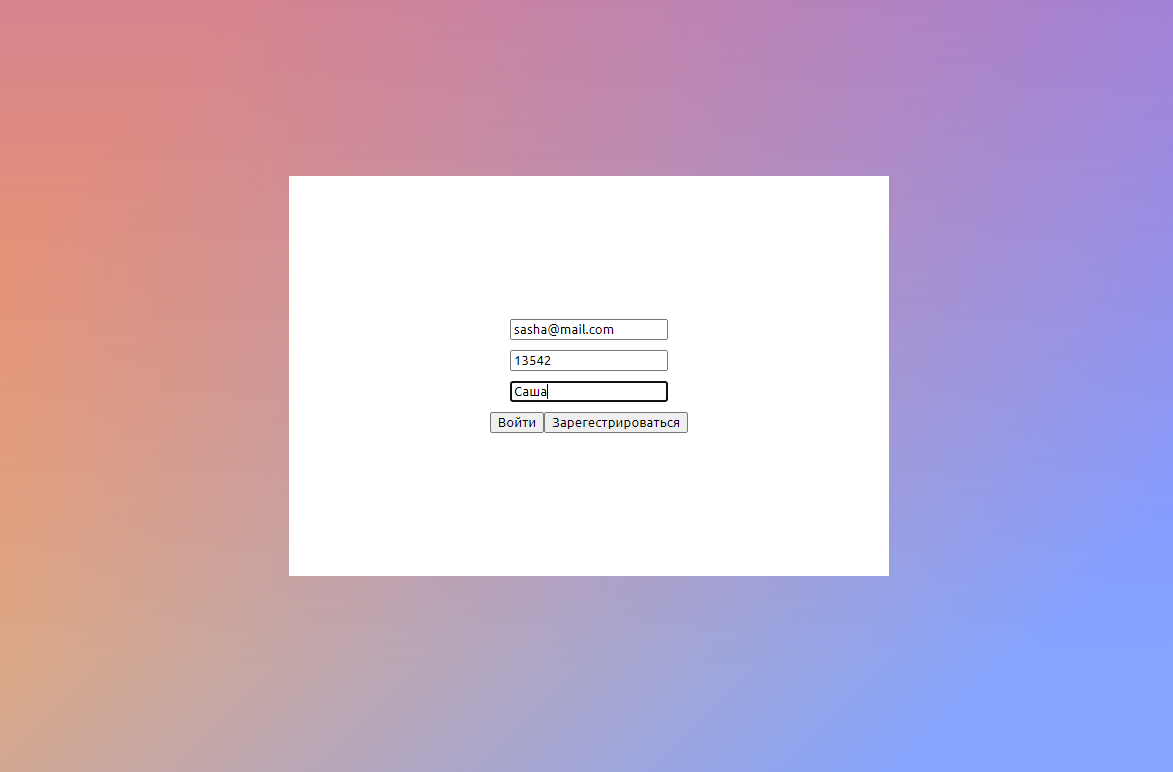
\includegraphics[width=14cm]{registr.png}
    \caption{Ввод данных пользователя для регистрации в системе}
    \label{fig:my_label}
\end{figure}
%\newline
После успешной авторизации пользователь попадает на главную страницу приложения. Дизайн данной страницы представлен на рисунке ниже (Рисунок \ref{fig:my_label1}).
\begin{figure}[H]
    \centering
    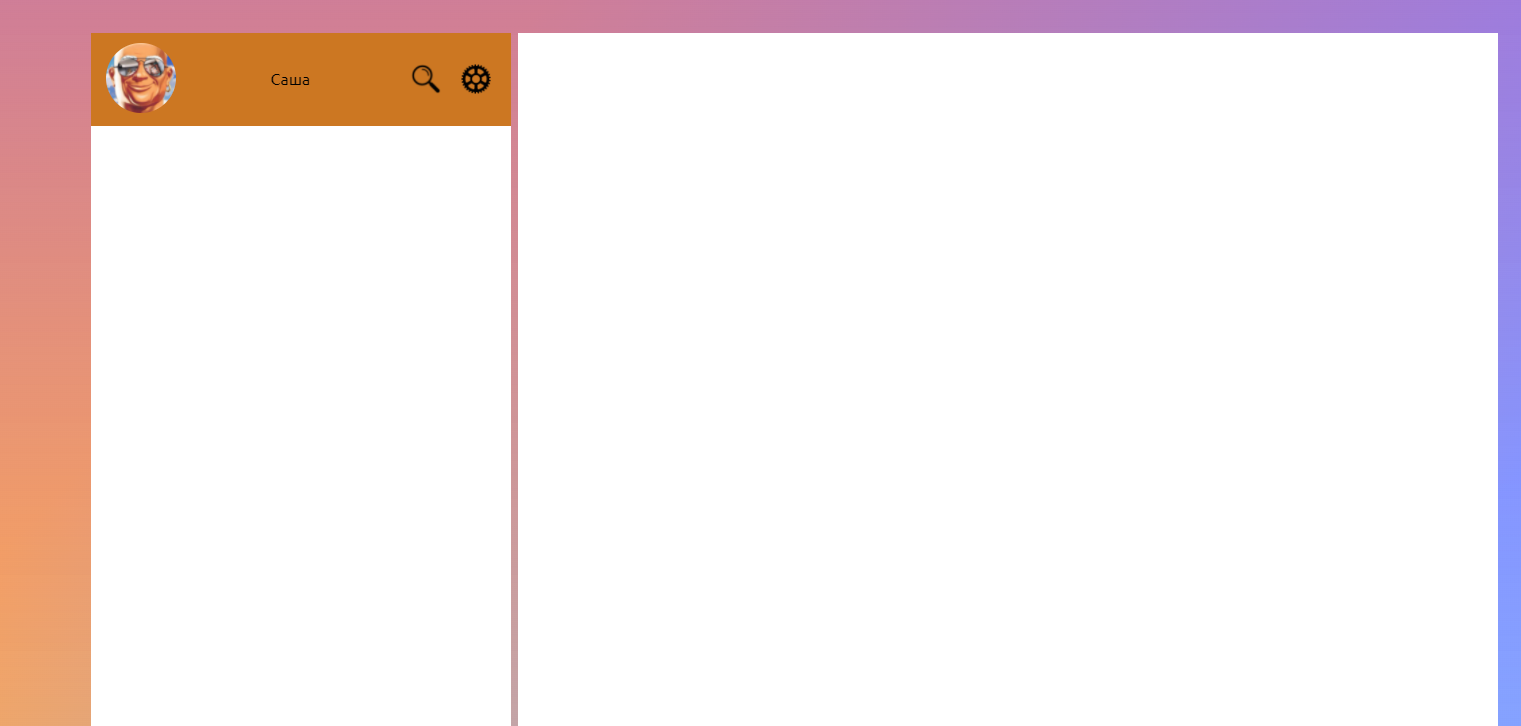
\includegraphics[width=14cm]{vhod.png}
    \caption{Главная страница приложения}
    \label{fig:my_label1}
\end{figure}
Слева находится боковое меню с мини профилем пользователя, а сразу под ним будет представлен список диалогов, которые на данный момент уже имеются у пользователя. В мини профиле меню находятся кнопки поиска пользователей, уже зарегистрированных в системе, а так же настроек, в которых можно изменить имя и аватар.
\par Справа находится основной блок, где будут представлены сообщения конкретного диалога, а так же форма для отправки сообщений.
\newline
\par
Самая главная функция мессенджера - это возможность пользователей обмениваться текстовыми сообщениями. Дизайн диалога двух пользователей можно посмотреть на картинках, представленных ниже (Рисунок \ref{fig:my_label2} и \ref{fig:my_label3} ). Справа, на основном блоке, расположено поле для ввода текста и рядом кнопка "Отправить". После отправки текстовое сообщение будет расположено справа в рамке фиолетового цвета - для пользователя отправившего данное сообщение и слева в рамке оранжевого цвета - для его собеседника. Сообщения пользователей располагаются сверху-вниз в соответствующих (правых и левых) столбцах.
\begin{figure}[H]
    \centering
    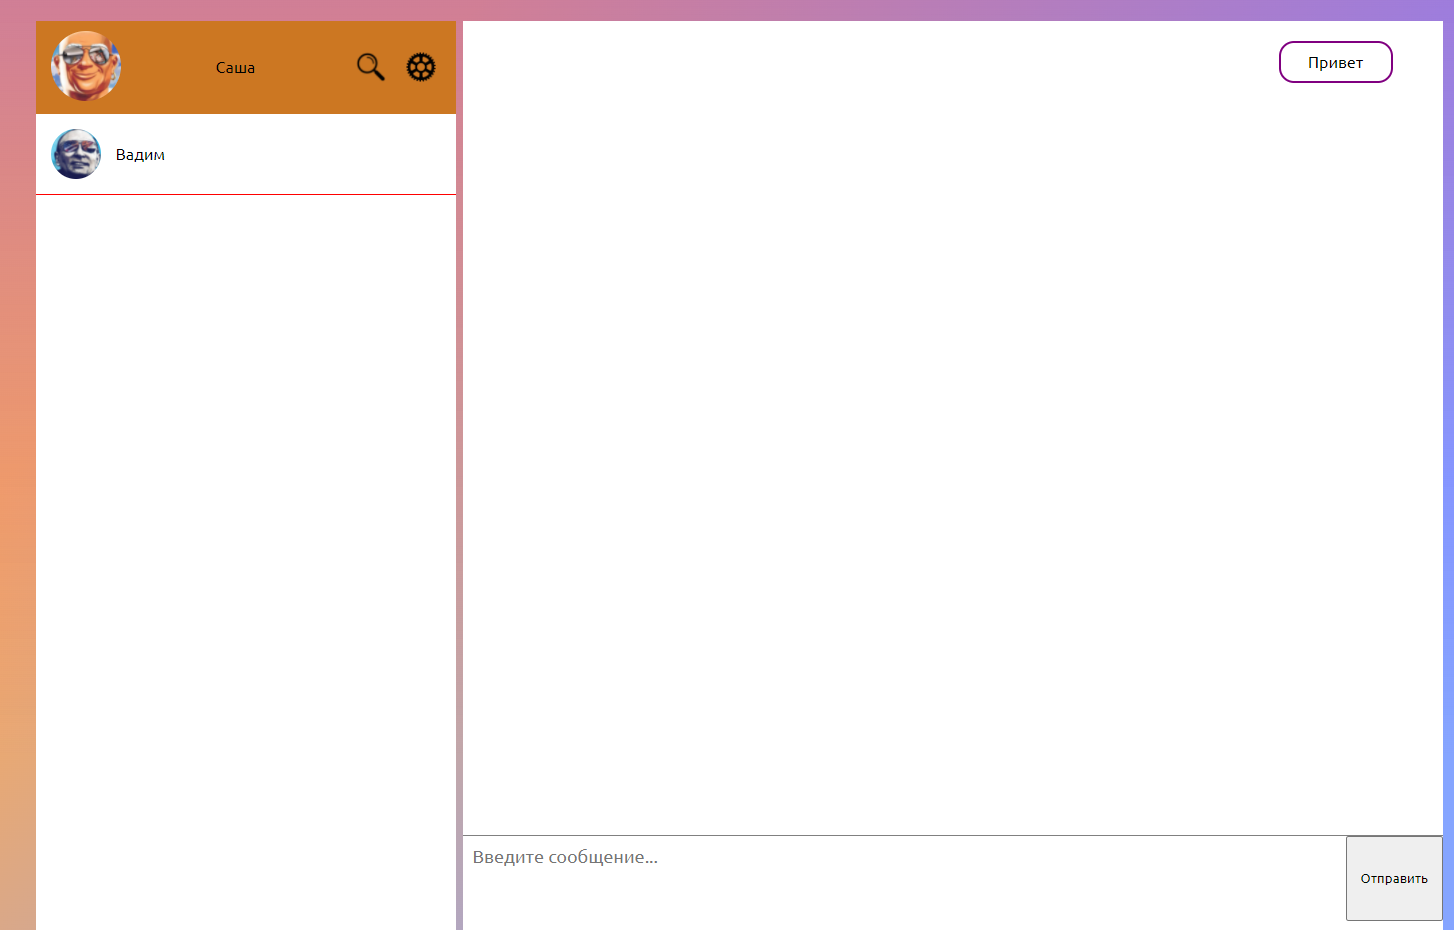
\includegraphics[width=14cm]{perepis.png}
    \caption{Вид диалога со стороны пользователя}
    \label{fig:my_label2}
\end{figure}
\begin{figure}[H]
    \centering
    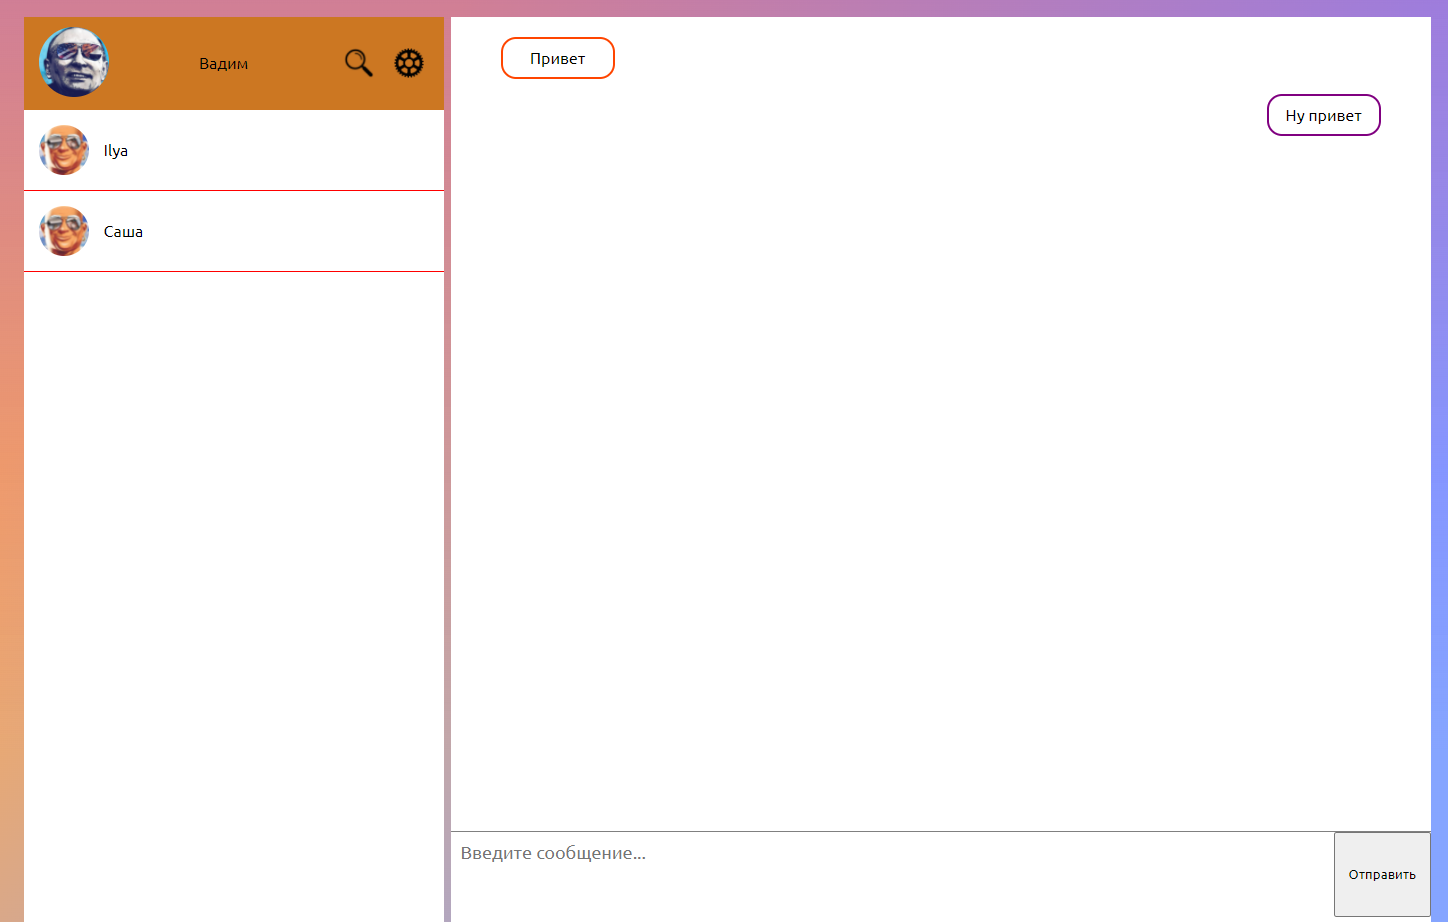
\includegraphics[width=14cm]{perepis1.png}
    \caption{Вид диалога со стороны собеседника}
    \label{fig:my_label3}
\end{figure}
\par
Приложение так же включает функцию изменения аватара и имени пользователя. Сделать это можно, нажав на "шестерёнку"  правее мини-профиля в левом углу окна приложения. При нажатии на данную кнопку - появляется два поля в центре страницы: для ввода нового имени; для ввода ссылки на картинку (Предназначено для изменения аватара в профиле). Справа от полей расположены кнопки с одинаковым названием "Применить" для установки соответствующего имени и (или) аватара (Рисунок \ref{fig:my_label4}).
\begin{figure}[H]
    \centering
    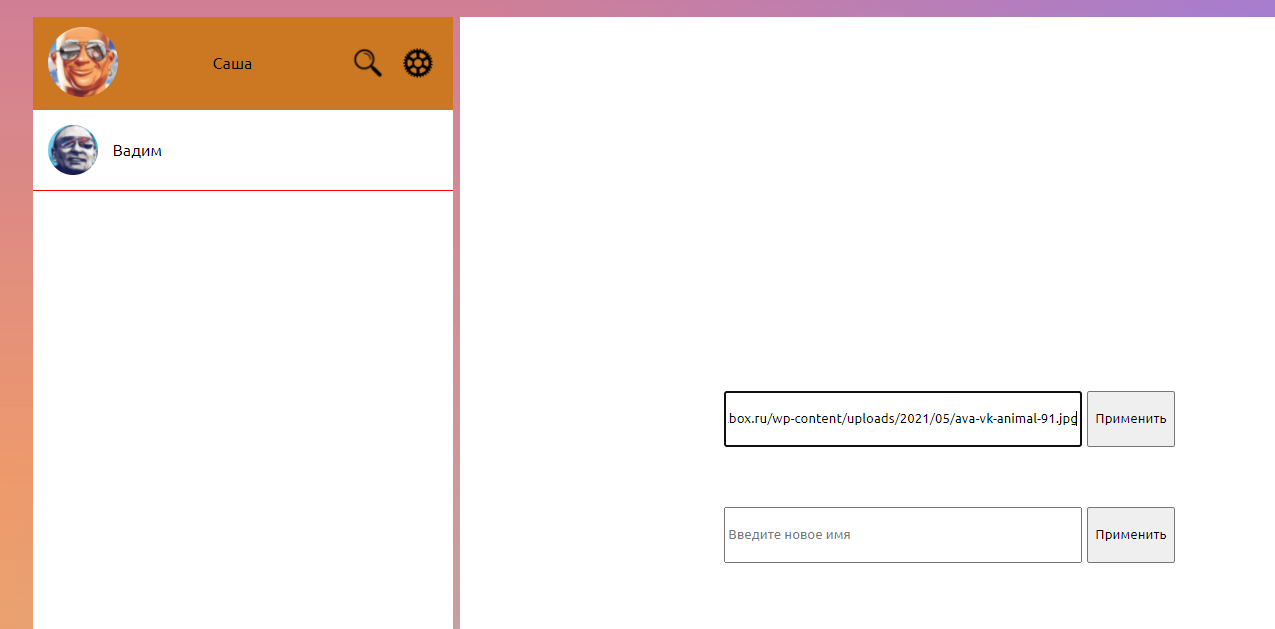
\includegraphics[width=13cm]{SmenaAvatara.png}
    \caption{Изменение настроек профиля}
    \label{fig:my_label4}
\end{figure}
\par
После ввода ссылки на картинку и нажатии на кнопку "Применить" аватар будет обновлен (Рисунок \ref{fig:my_label5}).
\begin{figure}[H]
    \centering
    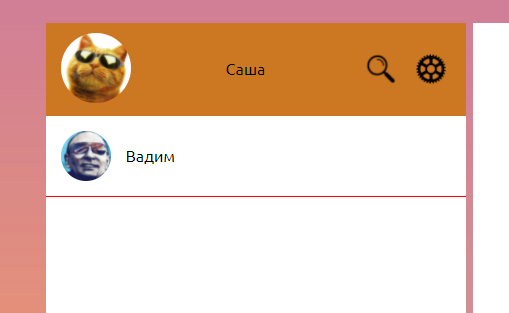
\includegraphics[width=13cm]{SmenaAvatara1.png}
    \caption{Обновленный аватар пользователя}
    \label{fig:my_label5}
\end{figure}
\par
Для поиска и добавления авторизованных пользователей в список диалогов создана кнопка в виде лупы, расположенная в мини-профиле пользователя в левом верхнем углу окна приложения. При нажатии на данную кнопку появляется поле для ввода Email-а пользователя в центре страницы, а так же кнопка "Найти"(Рисунок \ref{fig:my_label6}). После успешного поиска пользователя - собеседник будет добавлен в список диалогов ниже последнего, а при некорректном вводе Email или при отсутствии зарегистрированного по введённому Email пользователя будет выведено соответствующее сообщение об ошибке.
\begin{figure}[H]
    \centering
    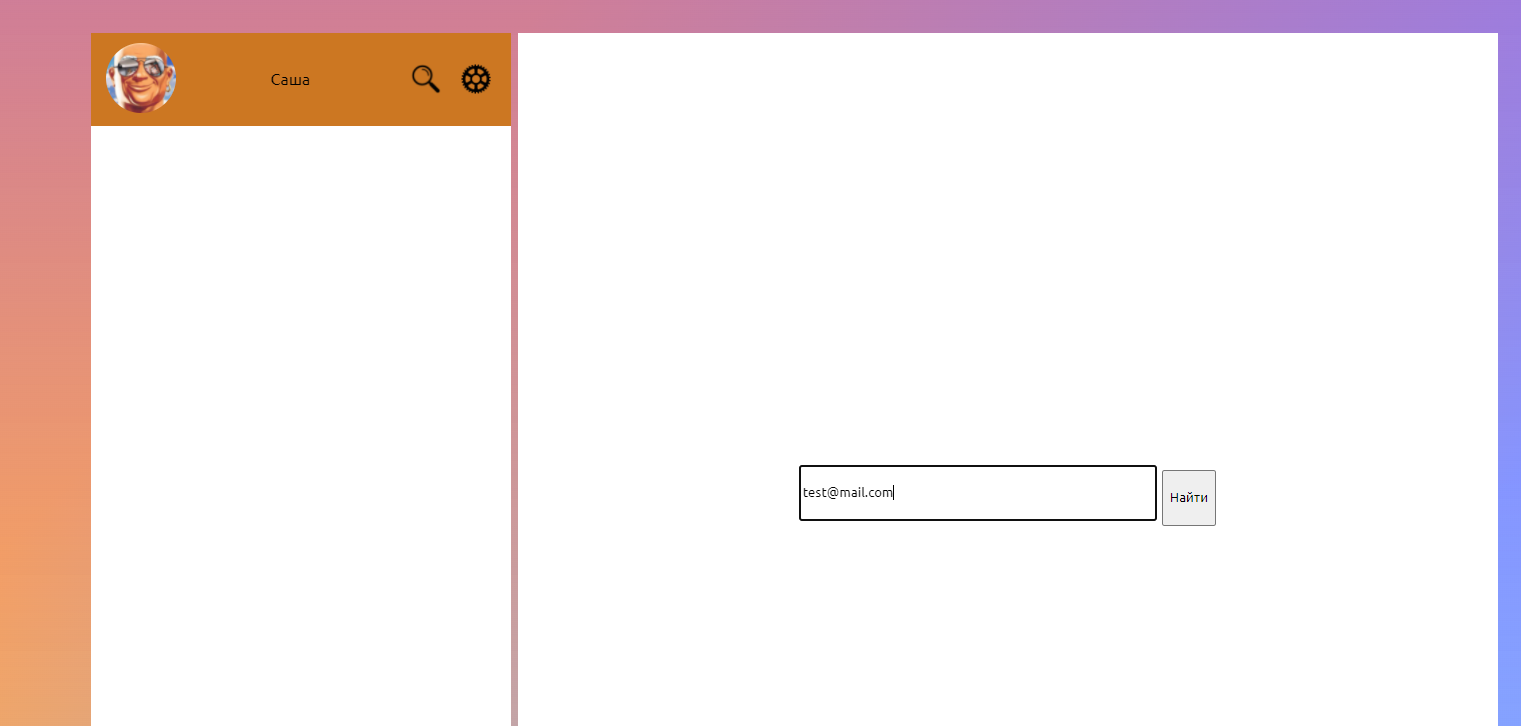
\includegraphics[width=13cm]{poisk.png}
    \caption{Ввод данных для добавления пользователя в список диалогов}
    \label{fig:my_label6}
\end{figure}
\par
Минимизация WEB-мессенджера влияет не только на скорость загрузки данных, но и помогает пользователю быстрее ориентироваться в приложении, именно поэтому разработан простой интерфейс, включающий в себя исключительно необходимые функции для использования WEB-мессенджера. 
\chapter*{ЗАКЛЮЧЕНИЕ}
В результате проделанной работы разработано WEB-приложение, представляющее собой простой WEB-мессенджер, позволяющий пользователям выполнять следующие операции:
\begin{itemize}
    \item Регистрироваться и авторизоваться в системе;
    \item Обмениваться текстовыми сообщениями;
    \item Изменять имя и аватар профиля;
    \item Осуществлять поиск собеседников через ввод Email
\end{itemize}
\par
Использование CSS-модулей позволило создать грамотную структуру сайта с красивым и хорошо подсознательно-воспринимаемым дизайном и удобную навигацию.
\par
Разработанный WEB-мессенджер можно доработать следующим образом:
\begin{enumerate}
    \item Получение сообщения без необходимости перезагрузки всего диалога;
    \item Возможность отправки файлов (картинок, аудио и др.);
    \item Возможность удаления сообщений и контактов;
    \item Отправку уведомлений в браузере;
    \item Зашифрованная отправка сообщений;
    \item Наличие отдельных таблиц в БД для хранения персональных данных.
\end{enumerate}

\begin{thebibliography}{99}
\bibitem{} Основы работы с CSS : учебное пособие. — 2-е изд. — Москва : ИНТУИТ, 2016. — 195 с.
\bibitem{} Тиге, Д. К. DHTML и CSS : учебное пособие / Д. К. Тиге. — Москва : ДМК Пресс, 2008. — 558 с.
\bibitem{} Хрусталев, А. А. Справочник CSS3. Кратко, быстро, под рукой : справочник / А. А. Хрусталев, Е. В. Дубовик. — Санкт-Петербург : Наука и Техника, 2021. — 304 с. 
\bibitem{} Кириченко, А. В. Web на практике. CSS, HTML, JavaScript, MySQL, PHP для fullstack-разработчиков / А. В. Кириченко, А. П. Никольский, Е. В. Дубовик. — Санкт-Петербург : Наука и Техника, 2021. — 432 с.
\end{thebibliography}

\appendices
\end{document}




%%% Local Variables:
%%% mode: latex
%%% TeX-master: t
%%% End:
